\documentclass{standalone}
\usepackage{tikz}
\usetikzlibrary{patterns, positioning}

\begin{document}
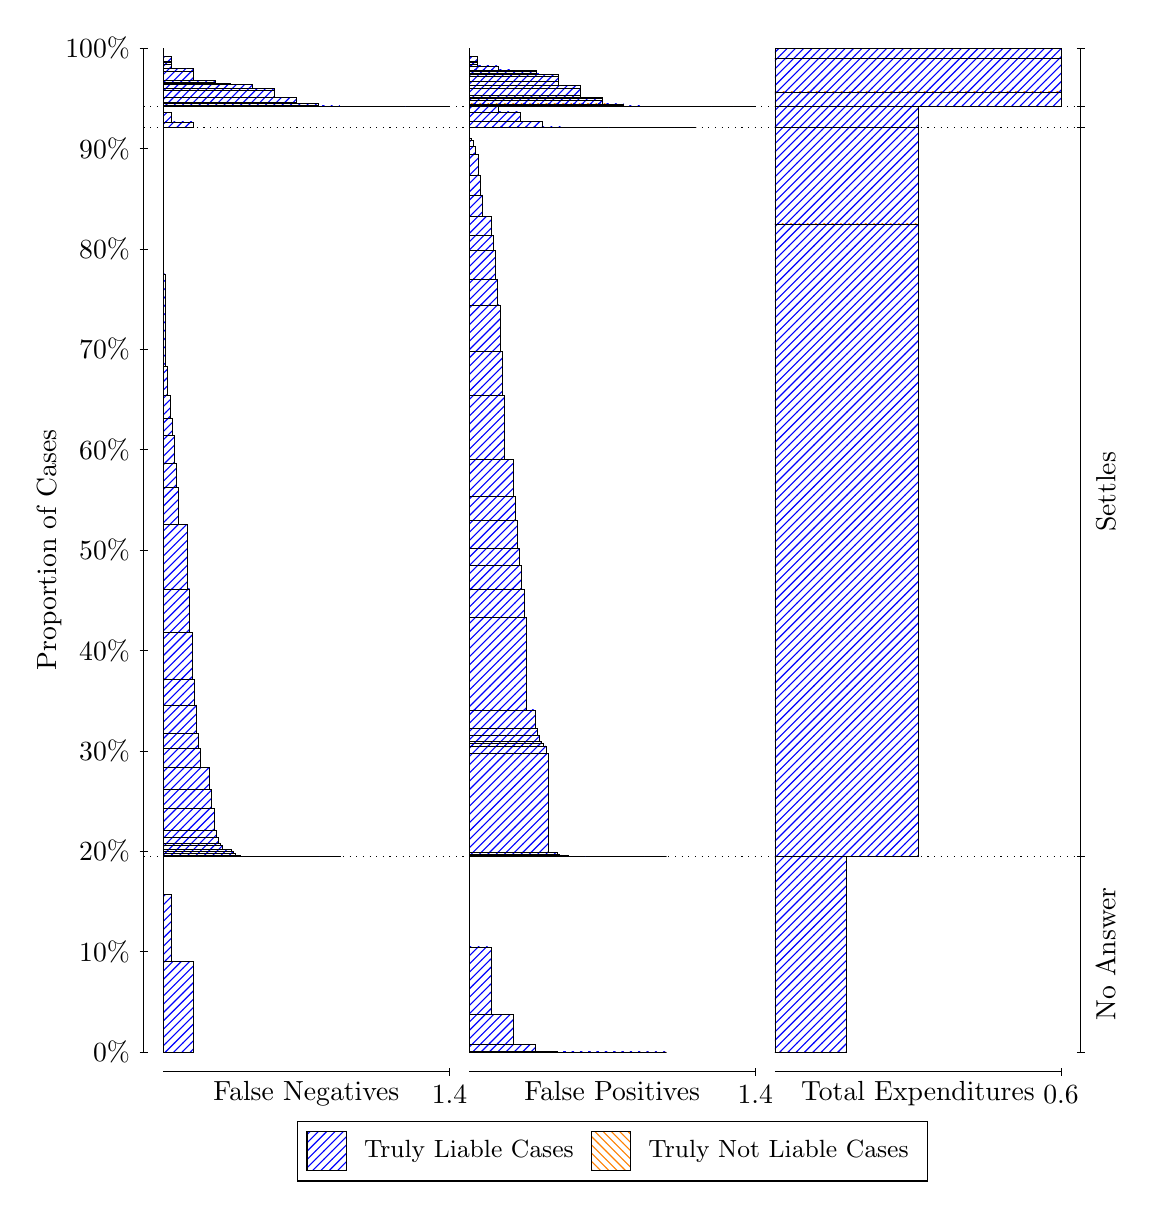
\begin{tikzpicture}
\draw[black, very thin] (1.5,1.75) -- (1.5,14.5);
\node[rotate=90, anchor=center] at (0.3, 8.125) {Proportion of Cases};
\draw[black, very thin] (1.45,1.75) -- (1.55,1.75);
\node[anchor=east] at (1.45, 1.75) {0\%};
\draw[black, very thin] (1.45,3.025) -- (1.55,3.025);
\node[anchor=east] at (1.45, 3.025) {10\%};
\draw[black, very thin] (1.45,4.3) -- (1.55,4.3);
\node[anchor=east] at (1.45, 4.3) {20\%};
\draw[black, very thin] (1.45,5.575) -- (1.55,5.575);
\node[anchor=east] at (1.45, 5.575) {30\%};
\draw[black, very thin] (1.45,6.85) -- (1.55,6.85);
\node[anchor=east] at (1.45, 6.85) {40\%};
\draw[black, very thin] (1.45,8.125) -- (1.55,8.125);
\node[anchor=east] at (1.45, 8.125) {50\%};
\draw[black, very thin] (1.45,9.4) -- (1.55,9.4);
\node[anchor=east] at (1.45, 9.4) {60\%};
\draw[black, very thin] (1.45,10.675) -- (1.55,10.675);
\node[anchor=east] at (1.45, 10.675) {70\%};
\draw[black, very thin] (1.45,11.95) -- (1.55,11.95);
\node[anchor=east] at (1.45, 11.95) {80\%};
\draw[black, very thin] (1.45,13.225) -- (1.55,13.225);
\node[anchor=east] at (1.45, 13.225) {90\%};
\draw[black, very thin] (1.45,14.5) -- (1.55,14.5);
\node[anchor=east] at (1.45, 14.5) {100\%};

\draw[black, very thin] (13.4,1.75) -- (13.4,14.5);
\draw[black, very thin] (13.35,1.75) -- (13.45,1.75);
\node[anchor=west] at (13.35, 1.75) {};
\draw[black, very thin] (13.35,4.2363) -- (13.45,4.2363);
\node[anchor=west] at (13.35, 4.2363) {};
\draw[black, very thin] (13.35,13.489) -- (13.45,13.489);
\node[anchor=west] at (13.35, 13.489) {};
\draw[black, very thin] (13.35,13.761) -- (13.45,13.761);
\node[anchor=west] at (13.35, 13.761) {};
\draw[black, very thin] (13.35,14.5) -- (13.45,14.5);
\node[anchor=west] at (13.35, 14.5) {};

\draw[black, very thin, pattern color=blue, pattern=north east lines] (1.75,1.75) rectangle (2.1259,2.9018);
\draw[black, very thin, pattern color=blue, pattern=north east lines] (1.75,2.9018) rectangle (1.8474,3.7553);
\draw[black, very thin, pattern color=orange, pattern=north west lines] (1.75,3.7553) rectangle (1.75,3.7553);
\draw[black, very thin, pattern color=blue, pattern=north east lines] (1.75,3.7553) rectangle (1.75,4.2363);
\draw[black, very thin, pattern color=blue, pattern=north east lines] (1.75,4.2363) rectangle (4.0052,4.2363);
\draw[black, very thin, pattern color=blue, pattern=north east lines] (1.75,4.2363) rectangle (3.7546,4.2363);
\draw[black, very thin, pattern color=blue, pattern=north east lines] (1.75,4.2363) rectangle (3.7268,4.2363);
\draw[black, very thin, pattern color=blue, pattern=north east lines] (1.75,4.2363) rectangle (3.504,4.2363);
\draw[black, very thin, pattern color=blue, pattern=north east lines] (1.75,4.2363) rectangle (3.4762,4.2363);
\draw[black, very thin, pattern color=blue, pattern=north east lines] (1.75,4.2363) rectangle (3.4483,4.2363);
\draw[black, very thin, pattern color=blue, pattern=north east lines] (1.75,4.2363) rectangle (3.2534,4.2363);
\draw[black, very thin, pattern color=blue, pattern=north east lines] (1.75,4.2363) rectangle (3.2256,4.2363);
\draw[black, very thin, pattern color=blue, pattern=north east lines] (1.75,4.2363) rectangle (3.1978,4.2363);
\draw[black, very thin, pattern color=blue, pattern=north east lines] (1.75,4.2363) rectangle (3.1699,4.2363);
\draw[black, very thin, pattern color=blue, pattern=north east lines] (1.75,4.2363) rectangle (3.0029,4.2364);
\draw[black, very thin, pattern color=blue, pattern=north east lines] (1.75,4.2364) rectangle (2.975,4.2364);
\draw[black, very thin, pattern color=blue, pattern=north east lines] (1.75,4.2364) rectangle (2.9472,4.237);
\draw[black, very thin, pattern color=blue, pattern=north east lines] (1.75,4.237) rectangle (2.9193,4.2375);
\draw[black, very thin, pattern color=blue, pattern=north east lines] (1.75,4.2375) rectangle (2.8915,4.238);
\draw[black, very thin, pattern color=blue, pattern=north east lines] (1.75,4.238) rectangle (2.7523,4.2391);
\draw[black, very thin, pattern color=blue, pattern=north east lines] (1.75,4.2391) rectangle (2.7245,4.2424);
\draw[black, very thin, pattern color=blue, pattern=north east lines] (1.75,4.2424) rectangle (2.6966,4.2478);
\draw[black, very thin, pattern color=blue, pattern=north east lines] (1.75,4.2478) rectangle (2.6688,4.2753);
\draw[black, very thin, pattern color=blue, pattern=north east lines] (1.75,4.2753) rectangle (2.6409,4.3011);
\draw[black, very thin, pattern color=blue, pattern=north east lines] (1.75,4.3011) rectangle (2.6131,4.3274);
\draw[black, very thin, pattern color=blue, pattern=north east lines] (1.75,4.3274) rectangle (2.5017,4.3725);
\draw[black, very thin, pattern color=blue, pattern=north east lines] (1.75,4.3725) rectangle (2.4739,4.3993);
\draw[black, very thin, pattern color=blue, pattern=north east lines] (1.75,4.3993) rectangle (2.446,4.4719);
\draw[black, very thin, pattern color=blue, pattern=north east lines] (1.75,4.4719) rectangle (2.4182,4.57);
\draw[black, very thin, pattern color=blue, pattern=north east lines] (1.75,4.57) rectangle (2.3904,4.8434);
\draw[black, very thin, pattern color=blue, pattern=north east lines] (1.75,4.8434) rectangle (2.3625,5.0892);
\draw[black, very thin, pattern color=blue, pattern=north east lines] (1.75,5.0892) rectangle (2.3347,5.361);
\draw[black, very thin, pattern color=blue, pattern=north east lines] (1.75,5.361) rectangle (2.2233,5.6035);
\draw[black, very thin, pattern color=blue, pattern=north east lines] (1.75,5.6035) rectangle (2.1955,5.7985);
\draw[black, very thin, pattern color=blue, pattern=north east lines] (1.75,5.7985) rectangle (2.1676,6.1574);
\draw[black, very thin, pattern color=blue, pattern=north east lines] (1.75,6.1574) rectangle (2.1398,6.4882);
\draw[black, very thin, pattern color=blue, pattern=north east lines] (1.75,6.4882) rectangle (2.1119,7.0807);
\draw[black, very thin, pattern color=blue, pattern=north east lines] (1.75,7.0807) rectangle (2.0841,7.6315);
\draw[black, very thin, pattern color=blue, pattern=north east lines] (1.75,7.6315) rectangle (2.0563,8.4516);
\draw[black, very thin, pattern color=blue, pattern=north east lines] (1.75,8.4516) rectangle (1.9449,8.9162);
\draw[black, very thin, pattern color=blue, pattern=north east lines] (1.75,8.9162) rectangle (1.917,9.2214);
\draw[black, very thin, pattern color=blue, pattern=north east lines] (1.75,9.2214) rectangle (1.8892,9.5802);
\draw[black, very thin, pattern color=blue, pattern=north east lines] (1.75,9.5802) rectangle (1.8614,9.7989);
\draw[black, very thin, pattern color=blue, pattern=north east lines] (1.75,9.7989) rectangle (1.8335,10.093);
\draw[black, very thin, pattern color=blue, pattern=north east lines] (1.75,10.093) rectangle (1.8057,10.455);
\draw[black, very thin, pattern color=blue, pattern=north east lines] (1.75,10.455) rectangle (1.7778,11.631);
\draw[black, very thin, pattern color=orange, pattern=north west lines] (1.75,11.631) rectangle (1.75,11.631);
\draw[black, very thin, pattern color=blue, pattern=north east lines] (1.75,11.631) rectangle (1.75,13.489);
\draw[black, very thin, pattern color=blue, pattern=north east lines] (1.75,13.489) rectangle (2.1259,13.562);
\draw[black, very thin, pattern color=blue, pattern=north east lines] (1.75,13.562) rectangle (1.8474,13.685);
\draw[black, very thin, pattern color=orange, pattern=north west lines] (1.75,13.685) rectangle (1.75,13.685);
\draw[black, very thin, pattern color=blue, pattern=north east lines] (1.75,13.685) rectangle (1.75,13.761);
\draw[black, very thin, pattern color=blue, pattern=north east lines] (1.75,13.761) rectangle (5.3833,13.761);
\draw[black, very thin, pattern color=blue, pattern=north east lines] (1.75,13.761) rectangle (5.1049,13.761);
\draw[black, very thin, pattern color=blue, pattern=north east lines] (1.75,13.761) rectangle (4.8265,13.761);
\draw[black, very thin, pattern color=blue, pattern=north east lines] (1.75,13.761) rectangle (4.8265,13.761);
\draw[black, very thin, pattern color=blue, pattern=north east lines] (1.75,13.761) rectangle (4.5481,13.761);
\draw[black, very thin, pattern color=blue, pattern=north east lines] (1.75,13.761) rectangle (4.2697,13.762);
\draw[black, very thin, pattern color=blue, pattern=north east lines] (1.75,13.762) rectangle (3.9913,13.766);
\draw[black, very thin, pattern color=blue, pattern=north east lines] (1.75,13.766) rectangle (3.7964,13.766);
\draw[black, very thin, pattern color=blue, pattern=north east lines] (1.75,13.766) rectangle (3.7128,13.776);
\draw[black, very thin, pattern color=blue, pattern=north east lines] (1.75,13.776) rectangle (3.7128,13.792);
\draw[black, very thin, pattern color=blue, pattern=north east lines] (1.75,13.792) rectangle (3.5179,13.792);
\draw[black, very thin, pattern color=blue, pattern=north east lines] (1.75,13.792) rectangle (3.5179,13.792);
\draw[black, very thin, pattern color=blue, pattern=north east lines] (1.75,13.792) rectangle (3.4344,13.809);
\draw[black, very thin, pattern color=blue, pattern=north east lines] (1.75,13.809) rectangle (3.4344,13.873);
\draw[black, very thin, pattern color=blue, pattern=north east lines] (1.75,13.873) rectangle (3.2395,13.873);
\draw[black, very thin, pattern color=blue, pattern=north east lines] (1.75,13.873) rectangle (3.156,13.963);
\draw[black, very thin, pattern color=blue, pattern=north east lines] (1.75,13.963) rectangle (3.156,13.989);
\draw[black, very thin, pattern color=blue, pattern=north east lines] (1.75,13.989) rectangle (2.9611,13.989);
\draw[black, very thin, pattern color=blue, pattern=north east lines] (1.75,13.989) rectangle (2.9611,13.989);
\draw[black, very thin, pattern color=blue, pattern=north east lines] (1.75,13.989) rectangle (2.8776,14.039);
\draw[black, very thin, pattern color=blue, pattern=north east lines] (1.75,14.039) rectangle (2.6827,14.042);
\draw[black, very thin, pattern color=blue, pattern=north east lines] (1.75,14.042) rectangle (2.5992,14.042);
\draw[black, very thin, pattern color=blue, pattern=north east lines] (1.75,14.042) rectangle (2.5992,14.045);
\draw[black, very thin, pattern color=blue, pattern=north east lines] (1.75,14.045) rectangle (2.5992,14.047);
\draw[black, very thin, pattern color=blue, pattern=north east lines] (1.75,14.047) rectangle (2.4043,14.063);
\draw[black, very thin, pattern color=blue, pattern=north east lines] (1.75,14.063) rectangle (2.4043,14.09);
\draw[black, very thin, pattern color=blue, pattern=north east lines] (1.75,14.09) rectangle (2.3208,14.091);
\draw[black, very thin, pattern color=blue, pattern=north east lines] (1.75,14.091) rectangle (2.3208,14.091);
\draw[black, very thin, pattern color=blue, pattern=north east lines] (1.75,14.091) rectangle (2.1259,14.206);
\draw[black, very thin, pattern color=blue, pattern=north east lines] (1.75,14.206) rectangle (2.1259,14.238);
\draw[black, very thin, pattern color=blue, pattern=north east lines] (1.75,14.238) rectangle (2.0423,14.238);
\draw[black, very thin, pattern color=blue, pattern=north east lines] (1.75,14.238) rectangle (2.0423,14.238);
\draw[black, very thin, pattern color=blue, pattern=north east lines] (1.75,14.238) rectangle (1.8474,14.29);
\draw[black, very thin, pattern color=blue, pattern=north east lines] (1.75,14.29) rectangle (1.8474,14.316);
\draw[black, very thin, pattern color=blue, pattern=north east lines] (1.75,14.316) rectangle (1.8474,14.329);
\draw[black, very thin, pattern color=blue, pattern=north east lines] (1.75,14.329) rectangle (1.8474,14.392);
\draw[black, very thin, pattern color=blue, pattern=north east lines] (1.75,14.392) rectangle (1.7639,14.392);
\draw[black, very thin, pattern color=blue, pattern=north east lines] (1.75,14.392) rectangle (1.7639,14.392);
\draw[black, very thin, pattern color=orange, pattern=north west lines] (1.75,14.392) rectangle (1.75,14.392);
\draw[black, very thin, pattern color=blue, pattern=north east lines] (1.75,14.392) rectangle (1.75,14.5);
\draw[black, very thin, pattern color=orange, pattern=north west lines] (5.6333,1.75) rectangle (8.1391,1.75);
\draw[black, very thin, pattern color=blue, pattern=north east lines] (5.6333,1.75) rectangle (8.1391,1.75);
\draw[black, very thin, pattern color=blue, pattern=north east lines] (5.6333,1.75) rectangle (7.8607,1.75);
\draw[black, very thin, pattern color=blue, pattern=north east lines] (5.6333,1.75) rectangle (7.5822,1.75);
\draw[black, very thin, pattern color=blue, pattern=north east lines] (5.6333,1.75) rectangle (7.3038,1.75);
\draw[black, very thin, pattern color=blue, pattern=north east lines] (5.6333,1.75) rectangle (7.0254,1.7503);
\draw[black, very thin, pattern color=blue, pattern=north east lines] (5.6333,1.7503) rectangle (6.747,1.7582);
\draw[black, very thin, pattern color=blue, pattern=north east lines] (5.6333,1.7582) rectangle (6.4686,1.8431);
\draw[black, very thin, pattern color=blue, pattern=north east lines] (5.6333,1.8431) rectangle (6.1902,2.231);
\draw[black, very thin, pattern color=blue, pattern=north east lines] (5.6333,2.231) rectangle (5.9117,3.0845);
\draw[black, very thin, pattern color=blue, pattern=north east lines] (5.6333,3.0845) rectangle (5.6333,4.2363);
\draw[black, very thin, pattern color=orange, pattern=north west lines] (5.6333,4.2363) rectangle (8.1391,4.2363);
\draw[black, very thin, pattern color=blue, pattern=north east lines] (5.6333,4.2363) rectangle (8.1391,4.2363);
\draw[black, very thin, pattern color=orange, pattern=north west lines] (5.6333,4.2363) rectangle (7.8885,4.2363);
\draw[black, very thin, pattern color=blue, pattern=north east lines] (5.6333,4.2363) rectangle (7.8885,4.2363);
\draw[black, very thin, pattern color=blue, pattern=north east lines] (5.6333,4.2363) rectangle (7.8607,4.2363);
\draw[black, very thin, pattern color=orange, pattern=north west lines] (5.6333,4.2363) rectangle (7.6379,4.2363);
\draw[black, very thin, pattern color=blue, pattern=north east lines] (5.6333,4.2363) rectangle (7.6379,4.2363);
\draw[black, very thin, pattern color=blue, pattern=north east lines] (5.6333,4.2363) rectangle (7.6101,4.2363);
\draw[black, very thin, pattern color=blue, pattern=north east lines] (5.6333,4.2363) rectangle (7.5822,4.2363);
\draw[black, very thin, pattern color=orange, pattern=north west lines] (5.6333,4.2363) rectangle (7.3874,4.2363);
\draw[black, very thin, pattern color=blue, pattern=north east lines] (5.6333,4.2363) rectangle (7.3874,4.2363);
\draw[black, very thin, pattern color=blue, pattern=north east lines] (5.6333,4.2363) rectangle (7.3595,4.2363);
\draw[black, very thin, pattern color=blue, pattern=north east lines] (5.6333,4.2363) rectangle (7.3317,4.2363);
\draw[black, very thin, pattern color=blue, pattern=north east lines] (5.6333,4.2363) rectangle (7.3038,4.2363);
\draw[black, very thin, pattern color=orange, pattern=north west lines] (5.6333,4.2363) rectangle (7.1368,4.2363);
\draw[black, very thin, pattern color=blue, pattern=north east lines] (5.6333,4.2363) rectangle (7.1368,4.2363);
\draw[black, very thin, pattern color=blue, pattern=north east lines] (5.6333,4.2363) rectangle (7.1089,4.2363);
\draw[black, very thin, pattern color=blue, pattern=north east lines] (5.6333,4.2363) rectangle (7.0811,4.2364);
\draw[black, very thin, pattern color=blue, pattern=north east lines] (5.6333,4.2364) rectangle (7.0533,4.2364);
\draw[black, very thin, pattern color=blue, pattern=north east lines] (5.6333,4.2364) rectangle (7.0254,4.2369);
\draw[black, very thin, pattern color=orange, pattern=north west lines] (5.6333,4.2369) rectangle (6.8862,4.2369);
\draw[black, very thin, pattern color=blue, pattern=north east lines] (5.6333,4.2369) rectangle (6.8862,4.2484);
\draw[black, very thin, pattern color=blue, pattern=north east lines] (5.6333,4.2484) rectangle (6.8584,4.2493);
\draw[black, very thin, pattern color=blue, pattern=north east lines] (5.6333,4.2493) rectangle (6.8305,4.2501);
\draw[black, very thin, pattern color=blue, pattern=north east lines] (5.6333,4.2501) rectangle (6.8027,4.2529);
\draw[black, very thin, pattern color=blue, pattern=north east lines] (5.6333,4.2529) rectangle (6.7748,4.2581);
\draw[black, very thin, pattern color=blue, pattern=north east lines] (5.6333,4.2581) rectangle (6.747,4.2833);
\draw[black, very thin, pattern color=orange, pattern=north west lines] (5.6333,4.2833) rectangle (6.6356,4.2833);
\draw[black, very thin, pattern color=blue, pattern=north east lines] (5.6333,4.2833) rectangle (6.6356,5.5464);
\draw[black, very thin, pattern color=blue, pattern=north east lines] (5.6333,5.5464) rectangle (6.6078,5.6367);
\draw[black, very thin, pattern color=blue, pattern=north east lines] (5.6333,5.6367) rectangle (6.5799,5.6699);
\draw[black, very thin, pattern color=blue, pattern=north east lines] (5.6333,5.6699) rectangle (6.5521,5.6987);
\draw[black, very thin, pattern color=blue, pattern=north east lines] (5.6333,5.6987) rectangle (6.5243,5.7704);
\draw[black, very thin, pattern color=blue, pattern=north east lines] (5.6333,5.7704) rectangle (6.4964,5.8636);
\draw[black, very thin, pattern color=blue, pattern=north east lines] (5.6333,5.8636) rectangle (6.4686,6.0948);
\draw[black, very thin, pattern color=blue, pattern=north east lines] (5.6333,6.0948) rectangle (6.3572,7.2707);
\draw[black, very thin, pattern color=blue, pattern=north east lines] (5.6333,7.2707) rectangle (6.3294,7.6325);
\draw[black, very thin, pattern color=blue, pattern=north east lines] (5.6333,7.6325) rectangle (6.3015,7.9268);
\draw[black, very thin, pattern color=blue, pattern=north east lines] (5.6333,7.9268) rectangle (6.2737,8.1455);
\draw[black, very thin, pattern color=blue, pattern=north east lines] (5.6333,8.1455) rectangle (6.2458,8.5043);
\draw[black, very thin, pattern color=blue, pattern=north east lines] (5.6333,8.5043) rectangle (6.218,8.8094);
\draw[black, very thin, pattern color=blue, pattern=north east lines] (5.6333,8.8094) rectangle (6.1902,9.2741);
\draw[black, very thin, pattern color=blue, pattern=north east lines] (5.6333,9.2741) rectangle (6.0788,10.094);
\draw[black, very thin, pattern color=blue, pattern=north east lines] (5.6333,10.094) rectangle (6.051,10.645);
\draw[black, very thin, pattern color=blue, pattern=north east lines] (5.6333,10.645) rectangle (6.0231,11.237);
\draw[black, very thin, pattern color=blue, pattern=north east lines] (5.6333,11.237) rectangle (5.9953,11.568);
\draw[black, very thin, pattern color=blue, pattern=north east lines] (5.6333,11.568) rectangle (5.9674,11.927);
\draw[black, very thin, pattern color=blue, pattern=north east lines] (5.6333,11.927) rectangle (5.9396,12.122);
\draw[black, very thin, pattern color=blue, pattern=north east lines] (5.6333,12.122) rectangle (5.9117,12.365);
\draw[black, very thin, pattern color=blue, pattern=north east lines] (5.6333,12.365) rectangle (5.8004,12.636);
\draw[black, very thin, pattern color=blue, pattern=north east lines] (5.6333,12.636) rectangle (5.7725,12.882);
\draw[black, very thin, pattern color=blue, pattern=north east lines] (5.6333,12.882) rectangle (5.7447,13.156);
\draw[black, very thin, pattern color=blue, pattern=north east lines] (5.6333,13.156) rectangle (5.7169,13.254);
\draw[black, very thin, pattern color=blue, pattern=north east lines] (5.6333,13.254) rectangle (5.689,13.326);
\draw[black, very thin, pattern color=blue, pattern=north east lines] (5.6333,13.326) rectangle (5.6612,13.353);
\draw[black, very thin, pattern color=blue, pattern=north east lines] (5.6333,13.353) rectangle (5.6333,13.489);
\draw[black, very thin, pattern color=orange, pattern=north west lines] (5.6333,13.489) rectangle (8.5149,13.489);
\draw[black, very thin, pattern color=blue, pattern=north east lines] (5.6333,13.489) rectangle (8.5149,13.489);
\draw[black, very thin, pattern color=blue, pattern=north east lines] (5.6333,13.489) rectangle (8.2365,13.489);
\draw[black, very thin, pattern color=blue, pattern=north east lines] (5.6333,13.489) rectangle (7.9581,13.489);
\draw[black, very thin, pattern color=blue, pattern=north east lines] (5.6333,13.489) rectangle (7.6797,13.489);
\draw[black, very thin, pattern color=blue, pattern=north east lines] (5.6333,13.489) rectangle (7.4013,13.489);
\draw[black, very thin, pattern color=blue, pattern=north east lines] (5.6333,13.489) rectangle (7.1229,13.49);
\draw[black, very thin, pattern color=blue, pattern=north east lines] (5.6333,13.49) rectangle (6.8444,13.499);
\draw[black, very thin, pattern color=blue, pattern=north east lines] (5.6333,13.499) rectangle (6.566,13.565);
\draw[black, very thin, pattern color=blue, pattern=north east lines] (5.6333,13.565) rectangle (6.2876,13.689);
\draw[black, very thin, pattern color=blue, pattern=north east lines] (5.6333,13.689) rectangle (6.0092,13.761);
\draw[black, very thin, pattern color=orange, pattern=north west lines] (5.6333,13.761) rectangle (9.2667,13.761);
\draw[black, very thin, pattern color=blue, pattern=north east lines] (5.6333,13.761) rectangle (9.2667,13.761);
\draw[black, very thin, pattern color=orange, pattern=north west lines] (5.6333,13.761) rectangle (8.9883,13.761);
\draw[black, very thin, pattern color=blue, pattern=north east lines] (5.6333,13.761) rectangle (8.9883,13.761);
\draw[black, very thin, pattern color=orange, pattern=north west lines] (5.6333,13.761) rectangle (8.7098,13.761);
\draw[black, very thin, pattern color=blue, pattern=north east lines] (5.6333,13.761) rectangle (8.7098,13.761);
\draw[black, very thin, pattern color=blue, pattern=north east lines] (5.6333,13.761) rectangle (8.7098,13.761);
\draw[black, very thin, pattern color=orange, pattern=north west lines] (5.6333,13.761) rectangle (8.4314,13.761);
\draw[black, very thin, pattern color=blue, pattern=north east lines] (5.6333,13.761) rectangle (8.4314,13.761);
\draw[black, very thin, pattern color=orange, pattern=north west lines] (5.6333,13.761) rectangle (8.153,13.761);
\draw[black, very thin, pattern color=blue, pattern=north east lines] (5.6333,13.761) rectangle (8.153,13.761);
\draw[black, very thin, pattern color=orange, pattern=north west lines] (5.6333,13.761) rectangle (7.9581,13.761);
\draw[black, very thin, pattern color=blue, pattern=north east lines] (5.6333,13.761) rectangle (7.9581,13.761);
\draw[black, very thin, pattern color=blue, pattern=north east lines] (5.6333,13.761) rectangle (7.8746,13.763);
\draw[black, very thin, pattern color=blue, pattern=north east lines] (5.6333,13.763) rectangle (7.8746,13.763);
\draw[black, very thin, pattern color=orange, pattern=north west lines] (5.6333,13.763) rectangle (7.8746,13.763);
\draw[black, very thin, pattern color=blue, pattern=north east lines] (5.6333,13.763) rectangle (7.8746,13.765);
\draw[black, very thin, pattern color=orange, pattern=north west lines] (5.6333,13.765) rectangle (7.6797,13.765);
\draw[black, very thin, pattern color=blue, pattern=north east lines] (5.6333,13.765) rectangle (7.6797,13.765);
\draw[black, very thin, pattern color=blue, pattern=north east lines] (5.6333,13.765) rectangle (7.5962,13.775);
\draw[black, very thin, pattern color=blue, pattern=north east lines] (5.6333,13.775) rectangle (7.5962,13.783);
\draw[black, very thin, pattern color=orange, pattern=north west lines] (5.6333,13.783) rectangle (7.5962,13.783);
\draw[black, very thin, pattern color=blue, pattern=north east lines] (5.6333,13.783) rectangle (7.5962,13.79);
\draw[black, very thin, pattern color=orange, pattern=north west lines] (5.6333,13.79) rectangle (7.4013,13.79);
\draw[black, very thin, pattern color=blue, pattern=north east lines] (5.6333,13.79) rectangle (7.4013,13.79);
\draw[black, very thin, pattern color=blue, pattern=north east lines] (5.6333,13.79) rectangle (7.4013,13.79);
\draw[black, very thin, pattern color=blue, pattern=north east lines] (5.6333,13.79) rectangle (7.3178,13.834);
\draw[black, very thin, pattern color=blue, pattern=north east lines] (5.6333,13.834) rectangle (7.3178,13.868);
\draw[black, very thin, pattern color=blue, pattern=north east lines] (5.6333,13.868) rectangle (7.3178,13.869);
\draw[black, very thin, pattern color=blue, pattern=north east lines] (5.6333,13.869) rectangle (7.1229,13.869);
\draw[black, very thin, pattern color=orange, pattern=north west lines] (5.6333,13.869) rectangle (7.1229,13.869);
\draw[black, very thin, pattern color=blue, pattern=north east lines] (5.6333,13.869) rectangle (7.1229,13.869);
\draw[black, very thin, pattern color=blue, pattern=north east lines] (5.6333,13.869) rectangle (7.0393,13.902);
\draw[black, very thin, pattern color=blue, pattern=north east lines] (5.6333,13.902) rectangle (7.0393,13.992);
\draw[black, very thin, pattern color=blue, pattern=north east lines] (5.6333,13.992) rectangle (7.0393,14.023);
\draw[black, very thin, pattern color=blue, pattern=north east lines] (5.6333,14.023) rectangle (6.8444,14.023);
\draw[black, very thin, pattern color=blue, pattern=north east lines] (5.6333,14.023) rectangle (6.8444,14.023);
\draw[black, very thin, pattern color=orange, pattern=north west lines] (5.6333,14.023) rectangle (6.8444,14.023);
\draw[black, very thin, pattern color=blue, pattern=north east lines] (5.6333,14.023) rectangle (6.8444,14.023);
\draw[black, very thin, pattern color=blue, pattern=north east lines] (5.6333,14.023) rectangle (6.7609,14.08);
\draw[black, very thin, pattern color=blue, pattern=north east lines] (5.6333,14.08) rectangle (6.7609,14.138);
\draw[black, very thin, pattern color=blue, pattern=north east lines] (5.6333,14.138) rectangle (6.7609,14.17);
\draw[black, very thin, pattern color=blue, pattern=north east lines] (5.6333,14.17) rectangle (6.566,14.17);
\draw[black, very thin, pattern color=orange, pattern=north west lines] (5.6333,14.17) rectangle (6.566,14.17);
\draw[black, very thin, pattern color=blue, pattern=north east lines] (5.6333,14.17) rectangle (6.566,14.171);
\draw[black, very thin, pattern color=blue, pattern=north east lines] (5.6333,14.171) rectangle (6.566,14.171);
\draw[black, very thin, pattern color=blue, pattern=north east lines] (5.6333,14.171) rectangle (6.4825,14.173);
\draw[black, very thin, pattern color=blue, pattern=north east lines] (5.6333,14.173) rectangle (6.4825,14.199);
\draw[black, very thin, pattern color=blue, pattern=north east lines] (5.6333,14.199) rectangle (6.4825,14.214);
\draw[black, very thin, pattern color=blue, pattern=north east lines] (5.6333,14.214) rectangle (6.2876,14.216);
\draw[black, very thin, pattern color=blue, pattern=north east lines] (5.6333,14.216) rectangle (6.2876,14.219);
\draw[black, very thin, pattern color=orange, pattern=north west lines] (5.6333,14.219) rectangle (6.2876,14.219);
\draw[black, very thin, pattern color=blue, pattern=north east lines] (5.6333,14.219) rectangle (6.2876,14.219);
\draw[black, very thin, pattern color=blue, pattern=north east lines] (5.6333,14.219) rectangle (6.2041,14.22);
\draw[black, very thin, pattern color=blue, pattern=north east lines] (5.6333,14.22) rectangle (6.2041,14.221);
\draw[black, very thin, pattern color=blue, pattern=north east lines] (5.6333,14.221) rectangle (6.2041,14.222);
\draw[black, very thin, pattern color=blue, pattern=north east lines] (5.6333,14.222) rectangle (6.0092,14.268);
\draw[black, very thin, pattern color=orange, pattern=north west lines] (5.6333,14.268) rectangle (6.0092,14.268);
\draw[black, very thin, pattern color=blue, pattern=north east lines] (5.6333,14.268) rectangle (6.0092,14.269);
\draw[black, very thin, pattern color=blue, pattern=north east lines] (5.6333,14.269) rectangle (6.0092,14.272);
\draw[black, very thin, pattern color=blue, pattern=north east lines] (5.6333,14.272) rectangle (5.9257,14.272);
\draw[black, very thin, pattern color=blue, pattern=north east lines] (5.6333,14.272) rectangle (5.9257,14.272);
\draw[black, very thin, pattern color=blue, pattern=north east lines] (5.6333,14.272) rectangle (5.7308,14.298);
\draw[black, very thin, pattern color=blue, pattern=north east lines] (5.6333,14.298) rectangle (5.7308,14.325);
\draw[black, very thin, pattern color=blue, pattern=north east lines] (5.6333,14.325) rectangle (5.7308,14.327);
\draw[black, very thin, pattern color=blue, pattern=north east lines] (5.6333,14.327) rectangle (5.7308,14.389);
\draw[black, very thin, pattern color=blue, pattern=north east lines] (5.6333,14.389) rectangle (5.6473,14.389);
\draw[black, very thin, pattern color=blue, pattern=north east lines] (5.6333,14.389) rectangle (5.6473,14.389);
\draw[black, very thin, pattern color=blue, pattern=north east lines] (5.6333,14.389) rectangle (5.6333,14.5);
\draw[black, very thin, pattern color=orange, pattern=north west lines] (9.5167,1.75) rectangle (10.425,1.75);
\draw[black, very thin, pattern color=blue, pattern=north east lines] (9.5167,1.75) rectangle (10.425,4.2363);
\draw[black, very thin, pattern color=orange, pattern=north west lines] (9.5167,4.2363) rectangle (11.333,4.2363);
\draw[black, very thin, pattern color=blue, pattern=north east lines] (9.5167,4.2363) rectangle (11.333,12.267);
\draw[black, very thin, pattern color=orange, pattern=north west lines] (9.5167,12.267) rectangle (11.333,12.267);
\draw[black, very thin, pattern color=blue, pattern=north east lines] (9.5167,12.267) rectangle (11.333,13.489);
\draw[black, very thin, pattern color=orange, pattern=north west lines] (9.5167,13.489) rectangle (11.333,13.489);
\draw[black, very thin, pattern color=blue, pattern=north east lines] (9.5167,13.489) rectangle (11.333,13.761);
\draw[black, very thin, pattern color=orange, pattern=north west lines] (9.5167,13.761) rectangle (13.15,13.761);
\draw[black, very thin, pattern color=blue, pattern=north east lines] (9.5167,13.761) rectangle (13.15,13.943);
\draw[black, very thin, pattern color=orange, pattern=north west lines] (9.5167,13.943) rectangle (13.15,13.943);
\draw[black, very thin, pattern color=blue, pattern=north east lines] (9.5167,13.943) rectangle (13.15,14.368);
\draw[black, very thin, pattern color=orange, pattern=north west lines] (9.5167,14.368) rectangle (13.15,14.368);
\draw[black, very thin, pattern color=blue, pattern=north east lines] (9.5167,14.368) rectangle (13.15,14.5);
\draw[black, dotted] (1.5,4.2363) -- (13.4,4.2363);
\draw[black, dotted] (1.5,13.489) -- (13.4,13.489);
\draw[black, dotted] (1.5,13.761) -- (13.4,13.761);
\draw[black, very thin] (1.75,1.5) -- (5.3833,1.5);
\node[anchor=north] at (3.5667, 1.5) {False Negatives};
\draw[black, very thin] (5.3833,1.45) -- (5.3833,1.55);
\node[anchor=north] at (5.3833, 1.45) {1.4};

\draw[black, very thin] (5.6333,1.5) -- (9.2667,1.5);
\node[anchor=north] at (7.45, 1.5) {False Positives};
\draw[black, very thin] (9.2667,1.45) -- (9.2667,1.55);
\node[anchor=north] at (9.2667, 1.45) {1.4};

\draw[black, very thin] (9.5167,1.5) -- (13.15,1.5);
\node[anchor=north] at (11.333, 1.5) {Total Expenditures};
\draw[black, very thin] (13.15,1.45) -- (13.15,1.55);
\node[anchor=north] at (13.15, 1.45) {0.6};

\node[black, centered, rotate=90] at (13.72, 2.9932) {No Answer};
\node[black, centered, rotate=90] at (13.72, 8.8628) {Settles};



\draw (7.449999999999999,1.5) node[draw=none] (baseCoordinate) {};
\begin{scope}[align=center]
        \matrix[scale=0.5, draw=black, below=0.5cm of baseCoordinate, nodes={draw}, column sep=0.1cm]{
            \node[rectangle, draw, minimum width=0.5cm, minimum height=0.5cm, pattern=north east lines, pattern color=blue] {}; &
            \node[draw=none, font=\small] (B) {Truly Liable Cases}; &
            \node[rectangle, draw, minimum width=0.5cm, minimum height=0.5cm, pattern=north west lines, pattern color=orange] {}; &
            \node[draw=none, font=\small] (B) {Truly Not Liable Cases}; \\
            };
\end{scope}

\end{tikzpicture}
\end{document}